% === Figure: Pareto scatter -- accuracy vs compute =========================
% The "lightweight beats heavy" money plot. y-axis = accuracy (CONFIRMED CTA
%   identical-protocol numbers); x-axis = compute.
% FLINT's compute is now a CONCRETE anchor: ~0.1 s CTA GBM fit + 46.4 KB model,
%   CPU (scripts/flint_efficiency.py). GRAMS+'s compute position is kept QUALITATIVE
%   /relative (heavier: GPU + 2 trained MLPs + Steiner search) -- we did NOT time
%   GRAMS+, so its x-coordinate is a relative placeholder, NOT a measured number.
% Standalone-includable: % === Figure: Pareto scatter -- accuracy vs compute =========================
% The "lightweight beats heavy" money plot. y-axis = accuracy (CONFIRMED CTA
%   identical-protocol numbers); x-axis = compute.
% FLINT's compute is now a CONCRETE anchor: ~0.1 s CTA GBM fit + 46.4 KB model,
%   CPU (scripts/flint_efficiency.py). GRAMS+'s compute position is kept QUALITATIVE
%   /relative (heavier: GPU + 2 trained MLPs + Steiner search) -- we did NOT time
%   GRAMS+, so its x-coordinate is a relative placeholder, NOT a measured number.
% Standalone-includable: % === Figure: Pareto scatter -- accuracy vs compute =========================
% The "lightweight beats heavy" money plot. y-axis = accuracy (CONFIRMED CTA
%   identical-protocol numbers); x-axis = compute.
% FLINT's compute is now a CONCRETE anchor: ~0.1 s CTA GBM fit + 46.4 KB model,
%   CPU (scripts/flint_efficiency.py). GRAMS+'s compute position is kept QUALITATIVE
%   /relative (heavier: GPU + 2 trained MLPs + Steiner search) -- we did NOT time
%   GRAMS+, so its x-coordinate is a relative placeholder, NOT a measured number.
% Standalone-includable: % === Figure: Pareto scatter -- accuracy vs compute =========================
% The "lightweight beats heavy" money plot. y-axis = accuracy (CONFIRMED CTA
%   identical-protocol numbers); x-axis = compute.
% FLINT's compute is now a CONCRETE anchor: ~0.1 s CTA GBM fit + 46.4 KB model,
%   CPU (scripts/flint_efficiency.py). GRAMS+'s compute position is kept QUALITATIVE
%   /relative (heavier: GPU + 2 trained MLPs + Steiner search) -- we did NOT time
%   GRAMS+, so its x-coordinate is a relative placeholder, NOT a measured number.
% Standalone-includable: \input{figures/pareto.tex} inside a figure environment.
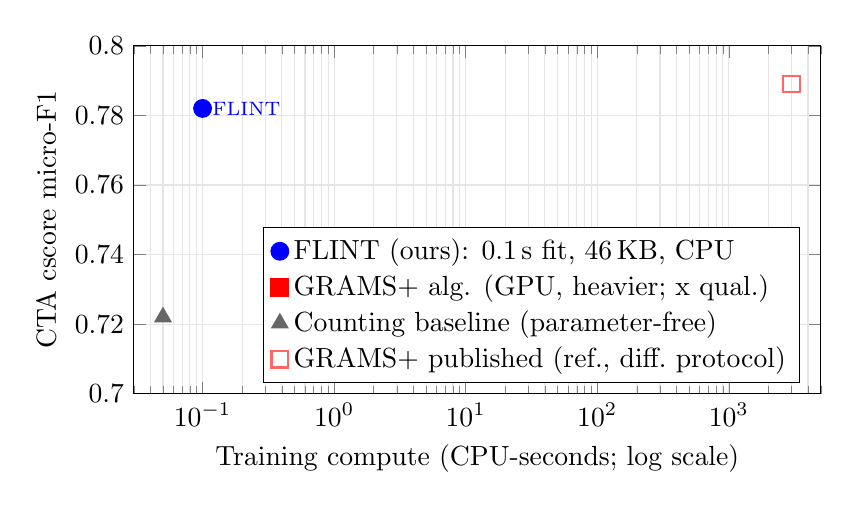
\begin{tikzpicture}
\begin{axis}[
    width=0.85\linewidth, height=6cm,
    xlabel={Training compute (CPU-seconds; log scale)},
    ylabel={CTA cscore micro-F1},
    xmode=log,
    xmin=0.03, xmax=5000,
    ymin=0.70, ymax=0.80,
    grid=both, grid style={gray!20},
    legend pos=south east,
    legend cell align=left,
    every axis plot/.append style={thick},
]
% FLINT: CONCRETE cost anchor -- 0.10 s CTA GBM fit (+ 46.4 KB model), CPU.
%   Placed at x=0.1 s (measured). High accuracy -> cheap-and-accurate corner.
\addplot[only marks, mark=*, mark size=3pt, color=blue]
    coordinates {(0.1, 0.782)};   % FLINT: 0.10 s CTA fit, 46.4 KB, CPU (MEASURED)
\addlegendentry{FLINT (ours): 0.1\,s fit, 46\,KB, CPU}
% GRAMS+ algorithm: heavier -- GPU + 2 trained MLPs + Steiner. x is a RELATIVE
%   placeholder (we did NOT time GRAMS+), shown only to convey "far to the right".
\addplot[only marks, mark=square*, mark size=3pt, color=red]
    coordinates {(2000, 0.732)}; % GRAMS+ algorithm (x RELATIVE/qualitative, not timed)
\addlegendentry{GRAMS+ alg. (GPU, heavier; x qual.)}
\addplot[only marks, mark=triangle*, mark size=3pt, color=black!60]
    coordinates {(0.05, 0.722)};  % counting baseline: parameter-free (relative)
\addlegendentry{Counting baseline (parameter-free)}
% reference: published GRAMS+ (different protocol/snapshot) as a hollow marker
\addplot[only marks, mark=square, mark size=3pt, color=red!60]
    coordinates {(3000, 0.789)}; % published GRAMS+ P2 (ref; different protocol)
\addlegendentry{GRAMS+ published (ref., diff.\ protocol)}
\node[anchor=west, font=\scriptsize, blue]   at (axis cs:0.1, 0.782) {FLINT};
\end{axis}
\end{tikzpicture}

% NOTE: FLINT's x-coordinate (0.1 s) is MEASURED (0.10 s CTA GBM fit on CPU; the
%   model is 46.4 KB; one-time frozen SBERT encode is 30.9 s, amortized and not a
%   per-run training cost). GRAMS+'s x-coordinate is a RELATIVE/qualitative placement
%   conveying "much heavier (GPU + two trained MLPs + Steiner search)"; it was NOT
%   timed and is not a fabricated wall-clock. y-values are CONFIRMED accuracy.
 inside a figure environment.
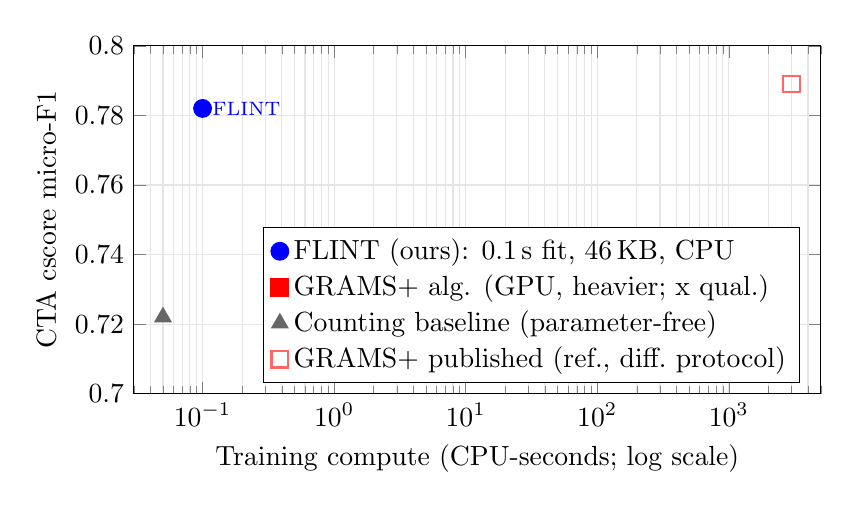
\begin{tikzpicture}
\begin{axis}[
    width=0.85\linewidth, height=6cm,
    xlabel={Training compute (CPU-seconds; log scale)},
    ylabel={CTA cscore micro-F1},
    xmode=log,
    xmin=0.03, xmax=5000,
    ymin=0.70, ymax=0.80,
    grid=both, grid style={gray!20},
    legend pos=south east,
    legend cell align=left,
    every axis plot/.append style={thick},
]
% FLINT: CONCRETE cost anchor -- 0.10 s CTA GBM fit (+ 46.4 KB model), CPU.
%   Placed at x=0.1 s (measured). High accuracy -> cheap-and-accurate corner.
\addplot[only marks, mark=*, mark size=3pt, color=blue]
    coordinates {(0.1, 0.782)};   % FLINT: 0.10 s CTA fit, 46.4 KB, CPU (MEASURED)
\addlegendentry{FLINT (ours): 0.1\,s fit, 46\,KB, CPU}
% GRAMS+ algorithm: heavier -- GPU + 2 trained MLPs + Steiner. x is a RELATIVE
%   placeholder (we did NOT time GRAMS+), shown only to convey "far to the right".
\addplot[only marks, mark=square*, mark size=3pt, color=red]
    coordinates {(2000, 0.732)}; % GRAMS+ algorithm (x RELATIVE/qualitative, not timed)
\addlegendentry{GRAMS+ alg. (GPU, heavier; x qual.)}
\addplot[only marks, mark=triangle*, mark size=3pt, color=black!60]
    coordinates {(0.05, 0.722)};  % counting baseline: parameter-free (relative)
\addlegendentry{Counting baseline (parameter-free)}
% reference: published GRAMS+ (different protocol/snapshot) as a hollow marker
\addplot[only marks, mark=square, mark size=3pt, color=red!60]
    coordinates {(3000, 0.789)}; % published GRAMS+ P2 (ref; different protocol)
\addlegendentry{GRAMS+ published (ref., diff.\ protocol)}
\node[anchor=west, font=\scriptsize, blue]   at (axis cs:0.1, 0.782) {FLINT};
\end{axis}
\end{tikzpicture}

% NOTE: FLINT's x-coordinate (0.1 s) is MEASURED (0.10 s CTA GBM fit on CPU; the
%   model is 46.4 KB; one-time frozen SBERT encode is 30.9 s, amortized and not a
%   per-run training cost). GRAMS+'s x-coordinate is a RELATIVE/qualitative placement
%   conveying "much heavier (GPU + two trained MLPs + Steiner search)"; it was NOT
%   timed and is not a fabricated wall-clock. y-values are CONFIRMED accuracy.
 inside a figure environment.
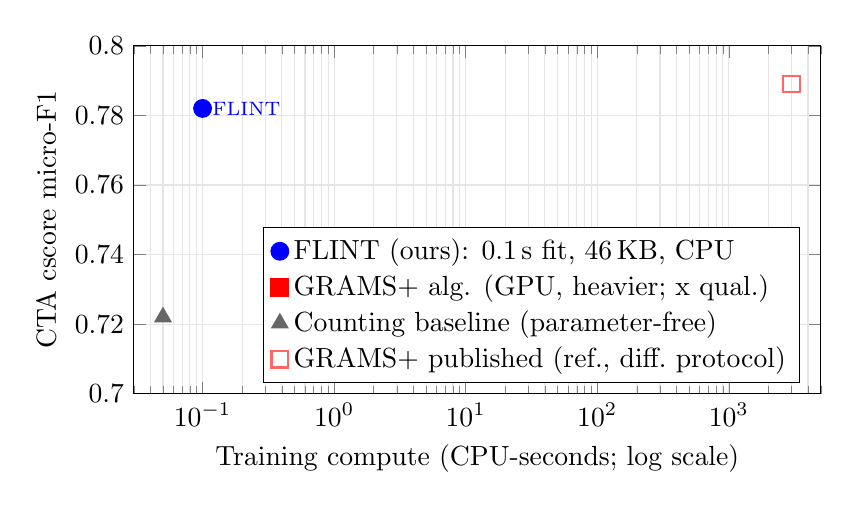
\begin{tikzpicture}
\begin{axis}[
    width=0.85\linewidth, height=6cm,
    xlabel={Training compute (CPU-seconds; log scale)},
    ylabel={CTA cscore micro-F1},
    xmode=log,
    xmin=0.03, xmax=5000,
    ymin=0.70, ymax=0.80,
    grid=both, grid style={gray!20},
    legend pos=south east,
    legend cell align=left,
    every axis plot/.append style={thick},
]
% FLINT: CONCRETE cost anchor -- 0.10 s CTA GBM fit (+ 46.4 KB model), CPU.
%   Placed at x=0.1 s (measured). High accuracy -> cheap-and-accurate corner.
\addplot[only marks, mark=*, mark size=3pt, color=blue]
    coordinates {(0.1, 0.782)};   % FLINT: 0.10 s CTA fit, 46.4 KB, CPU (MEASURED)
\addlegendentry{FLINT (ours): 0.1\,s fit, 46\,KB, CPU}
% GRAMS+ algorithm: heavier -- GPU + 2 trained MLPs + Steiner. x is a RELATIVE
%   placeholder (we did NOT time GRAMS+), shown only to convey "far to the right".
\addplot[only marks, mark=square*, mark size=3pt, color=red]
    coordinates {(2000, 0.732)}; % GRAMS+ algorithm (x RELATIVE/qualitative, not timed)
\addlegendentry{GRAMS+ alg. (GPU, heavier; x qual.)}
\addplot[only marks, mark=triangle*, mark size=3pt, color=black!60]
    coordinates {(0.05, 0.722)};  % counting baseline: parameter-free (relative)
\addlegendentry{Counting baseline (parameter-free)}
% reference: published GRAMS+ (different protocol/snapshot) as a hollow marker
\addplot[only marks, mark=square, mark size=3pt, color=red!60]
    coordinates {(3000, 0.789)}; % published GRAMS+ P2 (ref; different protocol)
\addlegendentry{GRAMS+ published (ref., diff.\ protocol)}
\node[anchor=west, font=\scriptsize, blue]   at (axis cs:0.1, 0.782) {FLINT};
\end{axis}
\end{tikzpicture}

% NOTE: FLINT's x-coordinate (0.1 s) is MEASURED (0.10 s CTA GBM fit on CPU; the
%   model is 46.4 KB; one-time frozen SBERT encode is 30.9 s, amortized and not a
%   per-run training cost). GRAMS+'s x-coordinate is a RELATIVE/qualitative placement
%   conveying "much heavier (GPU + two trained MLPs + Steiner search)"; it was NOT
%   timed and is not a fabricated wall-clock. y-values are CONFIRMED accuracy.
 inside a figure environment.
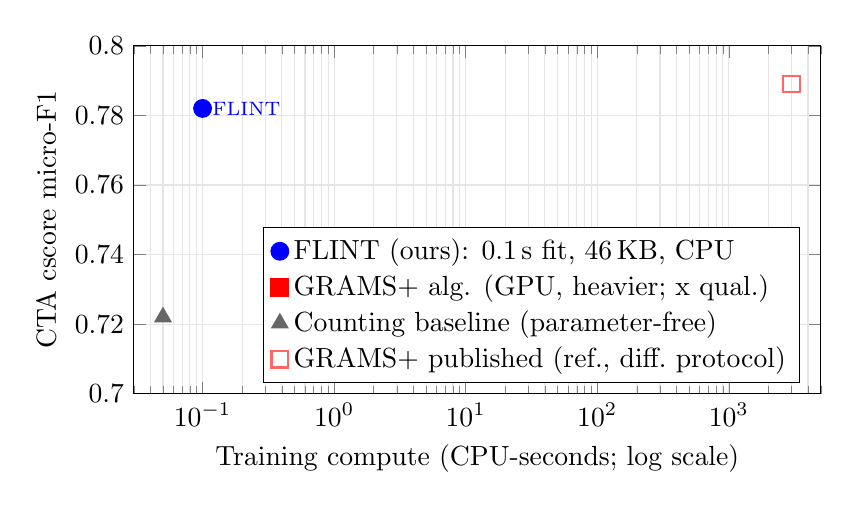
\begin{tikzpicture}
\begin{axis}[
    width=0.85\linewidth, height=6cm,
    xlabel={Training compute (CPU-seconds; log scale)},
    ylabel={CTA cscore micro-F1},
    xmode=log,
    xmin=0.03, xmax=5000,
    ymin=0.70, ymax=0.80,
    grid=both, grid style={gray!20},
    legend pos=south east,
    legend cell align=left,
    every axis plot/.append style={thick},
]
% FLINT: CONCRETE cost anchor -- 0.10 s CTA GBM fit (+ 46.4 KB model), CPU.
%   Placed at x=0.1 s (measured). High accuracy -> cheap-and-accurate corner.
\addplot[only marks, mark=*, mark size=3pt, color=blue]
    coordinates {(0.1, 0.782)};   % FLINT: 0.10 s CTA fit, 46.4 KB, CPU (MEASURED)
\addlegendentry{FLINT (ours): 0.1\,s fit, 46\,KB, CPU}
% GRAMS+ algorithm: heavier -- GPU + 2 trained MLPs + Steiner. x is a RELATIVE
%   placeholder (we did NOT time GRAMS+), shown only to convey "far to the right".
\addplot[only marks, mark=square*, mark size=3pt, color=red]
    coordinates {(2000, 0.732)}; % GRAMS+ algorithm (x RELATIVE/qualitative, not timed)
\addlegendentry{GRAMS+ alg. (GPU, heavier; x qual.)}
\addplot[only marks, mark=triangle*, mark size=3pt, color=black!60]
    coordinates {(0.05, 0.722)};  % counting baseline: parameter-free (relative)
\addlegendentry{Counting baseline (parameter-free)}
% reference: published GRAMS+ (different protocol/snapshot) as a hollow marker
\addplot[only marks, mark=square, mark size=3pt, color=red!60]
    coordinates {(3000, 0.789)}; % published GRAMS+ P2 (ref; different protocol)
\addlegendentry{GRAMS+ published (ref., diff.\ protocol)}
\node[anchor=west, font=\scriptsize, blue]   at (axis cs:0.1, 0.782) {FLINT};
\end{axis}
\end{tikzpicture}

% NOTE: FLINT's x-coordinate (0.1 s) is MEASURED (0.10 s CTA GBM fit on CPU; the
%   model is 46.4 KB; one-time frozen SBERT encode is 30.9 s, amortized and not a
%   per-run training cost). GRAMS+'s x-coordinate is a RELATIVE/qualitative placement
%   conveying "much heavier (GPU + two trained MLPs + Steiner search)"; it was NOT
%   timed and is not a fabricated wall-clock. y-values are CONFIRMED accuracy.
